\chapter{Praktischer Teil}
\label{chapter_Praktischer_Teil}
In diesem Kapitel werden die verschiedenen Sensorschaltungen und deren Konfiguration, die Problem
die sich bei der Realisierung ergaben, sowie die Ergebnisse und Auswertungen beschrieben. Außerdem werden die verschiedenen Möglichkeiten zur Datenspeicherung und Visualisierung dargestellt und erklärt. Am Anfang dieses Kapitels werden die zur Realisierung der verschiedenen Aufgaben benötigten Bauteile, kurz etwas näher erklärt und aufgelistet. In Abschnitt \ref{section_DS18S20} wird eine Schaltung mit einem einzigen 1-Wire Temperatursensor aufgebaut, bei der zweiten Schaltung in Abschnitt \ref{section_HTY221} kommt zu dem Sensor aus \ref{section_DS18S20} ein zweiter Temperatursensor und ein Sensor zur Temperatur- und Luftfeuchtigkeitsmessung hinzu. Der letzte Abschnitt (\ref{section_BMA020}) befasst sich mit der Realisierung einer Vibrationsmessung mittels Beschleunigungssensors.

\section{Benötigte Materialien}
\label{section_Benötigte_Materialien}
Die in Tabelle aufgelisteten Materialien wurden für die in Kapitel \ref{chapter_Praktischer_Teil} beschriebenen Versuche verwendet. In den jeweiligen Abschnitten, werden die  einzelnen Sensoren mit deren wichtigsten Technischen Daten noch genauer erklärt. 

%Tabelle 1
\begin{table}[H]
%\rowcolors{2}{black!10}{black!20}
\centering
\begin{tabular}{
lc
}
\toprule
\multicolumn{1}{p{6cm}}{\textit{Bezeichnung}} & \multicolumn{1}{p{3.5cm}}{\centering\textit{Anzahl} } \\\midrule
Raspberry Pi\,3& 1 \\
&\\
Temperatursensor DS18S20 & 2 \\
&\\
Sensor HYT\,221 & 1\\
&\\
3-Achsen-Beschleunigungssensor & 1\\
&\\
Drahtbrücken & mehrere\\
&\\
elektrischer Widerstand 4.7\,$k\Omega$ & 1\\
&\\
Elektronik Steckbrett & 1\\
\bottomrule
\end{tabular}
\caption{benötigte Materialien}
\label{Tabelle_benötigte_Materialien}
\end{table}

%Abschnitt DS18S20
\section{Temperaturmessung mit Sensor DS18S20}
\label{section_DS18S20}
Abschnitt \ref{section_DS18S20} befasst sich mit dem Schaltungsaufbau zur Temperaturmessung mittels DS18S20. Hier wird auf die Möglichkeit der Datenspeicherung und Visualisierung der Daten mit dem RRDtool eingegangen.
 

\subsection{DS18S20}
\label{subsection_DS18S20}
Der DS18S20 (siehe Abbildung \ref{Abb_DS18S20}) ist ein digitaler 1-Wire Temperatursensor, der eine Temperaturmessung mit 9\,Bit Auflösung ermöglicht. Dieser ist von der Firma \textit{Maxim Integrated} entwickelt worden.
Folgend werden die wichtigsten technischen Daten des DB18S20 aufgeführt.

%Abbildund Daten DS18S20
\begin{figure}[!h] 
  \centering
     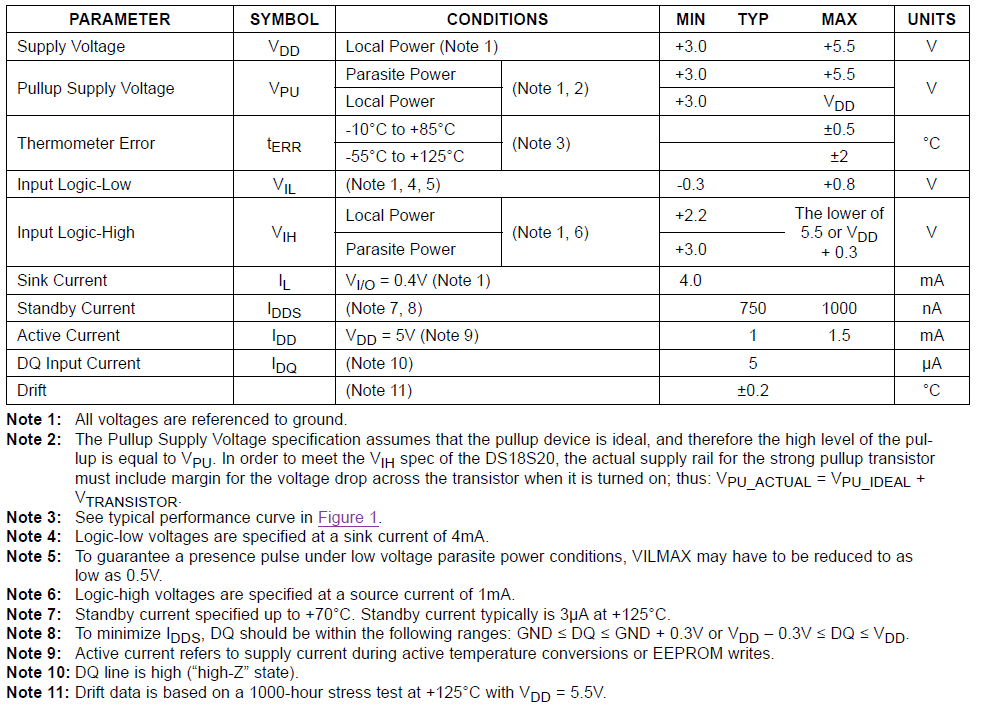
\includegraphics[scale=.6]{BilderAllgemein/Daten_DB18S20.png}
  \caption{elektische Daten DB18S20 \citep[S. 2]{Datenblatt_DB18S20}}
  \label{Abb_elektrische_Daten_DS18S20}
\end{figure}

%Abbildund  DS18S20
\begin{figure}[!h] 
  \centering
     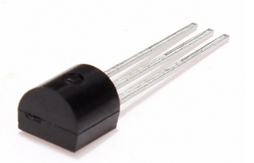
\includegraphics[scale=.4]{BilderAllgemein/DS18S20.png}
  \caption{DS18S20 \citep{Bild_DS18S20}}
  \label{Abb_DS18S20}
\end{figure}

\subsection{Schaltungsaufbau}
\label{subsection_Schaltungsaufbau_DS18S20}

Abbildung \ref{Abb_Schaltung_DS18S20} zeigt den schematischen Schaltungsaufbau mit dem Temperatursensor DS18S20. Anzumerken ist, dass die in der Schaltung in Abbildung \ref{Abb_Schaltung_DS18S20} dargestellten Bauteile optisch nicht immer den realen Bauteilen entsprechen (z.B. Form, Farbe oder Aufdruck). Die Beschaltung der Bauteile ist jedoch korrekt dargestellt. 

%Abbildund Schaltungsaufbau DS18S20
\begin{figure}[!h] 
  \centering
     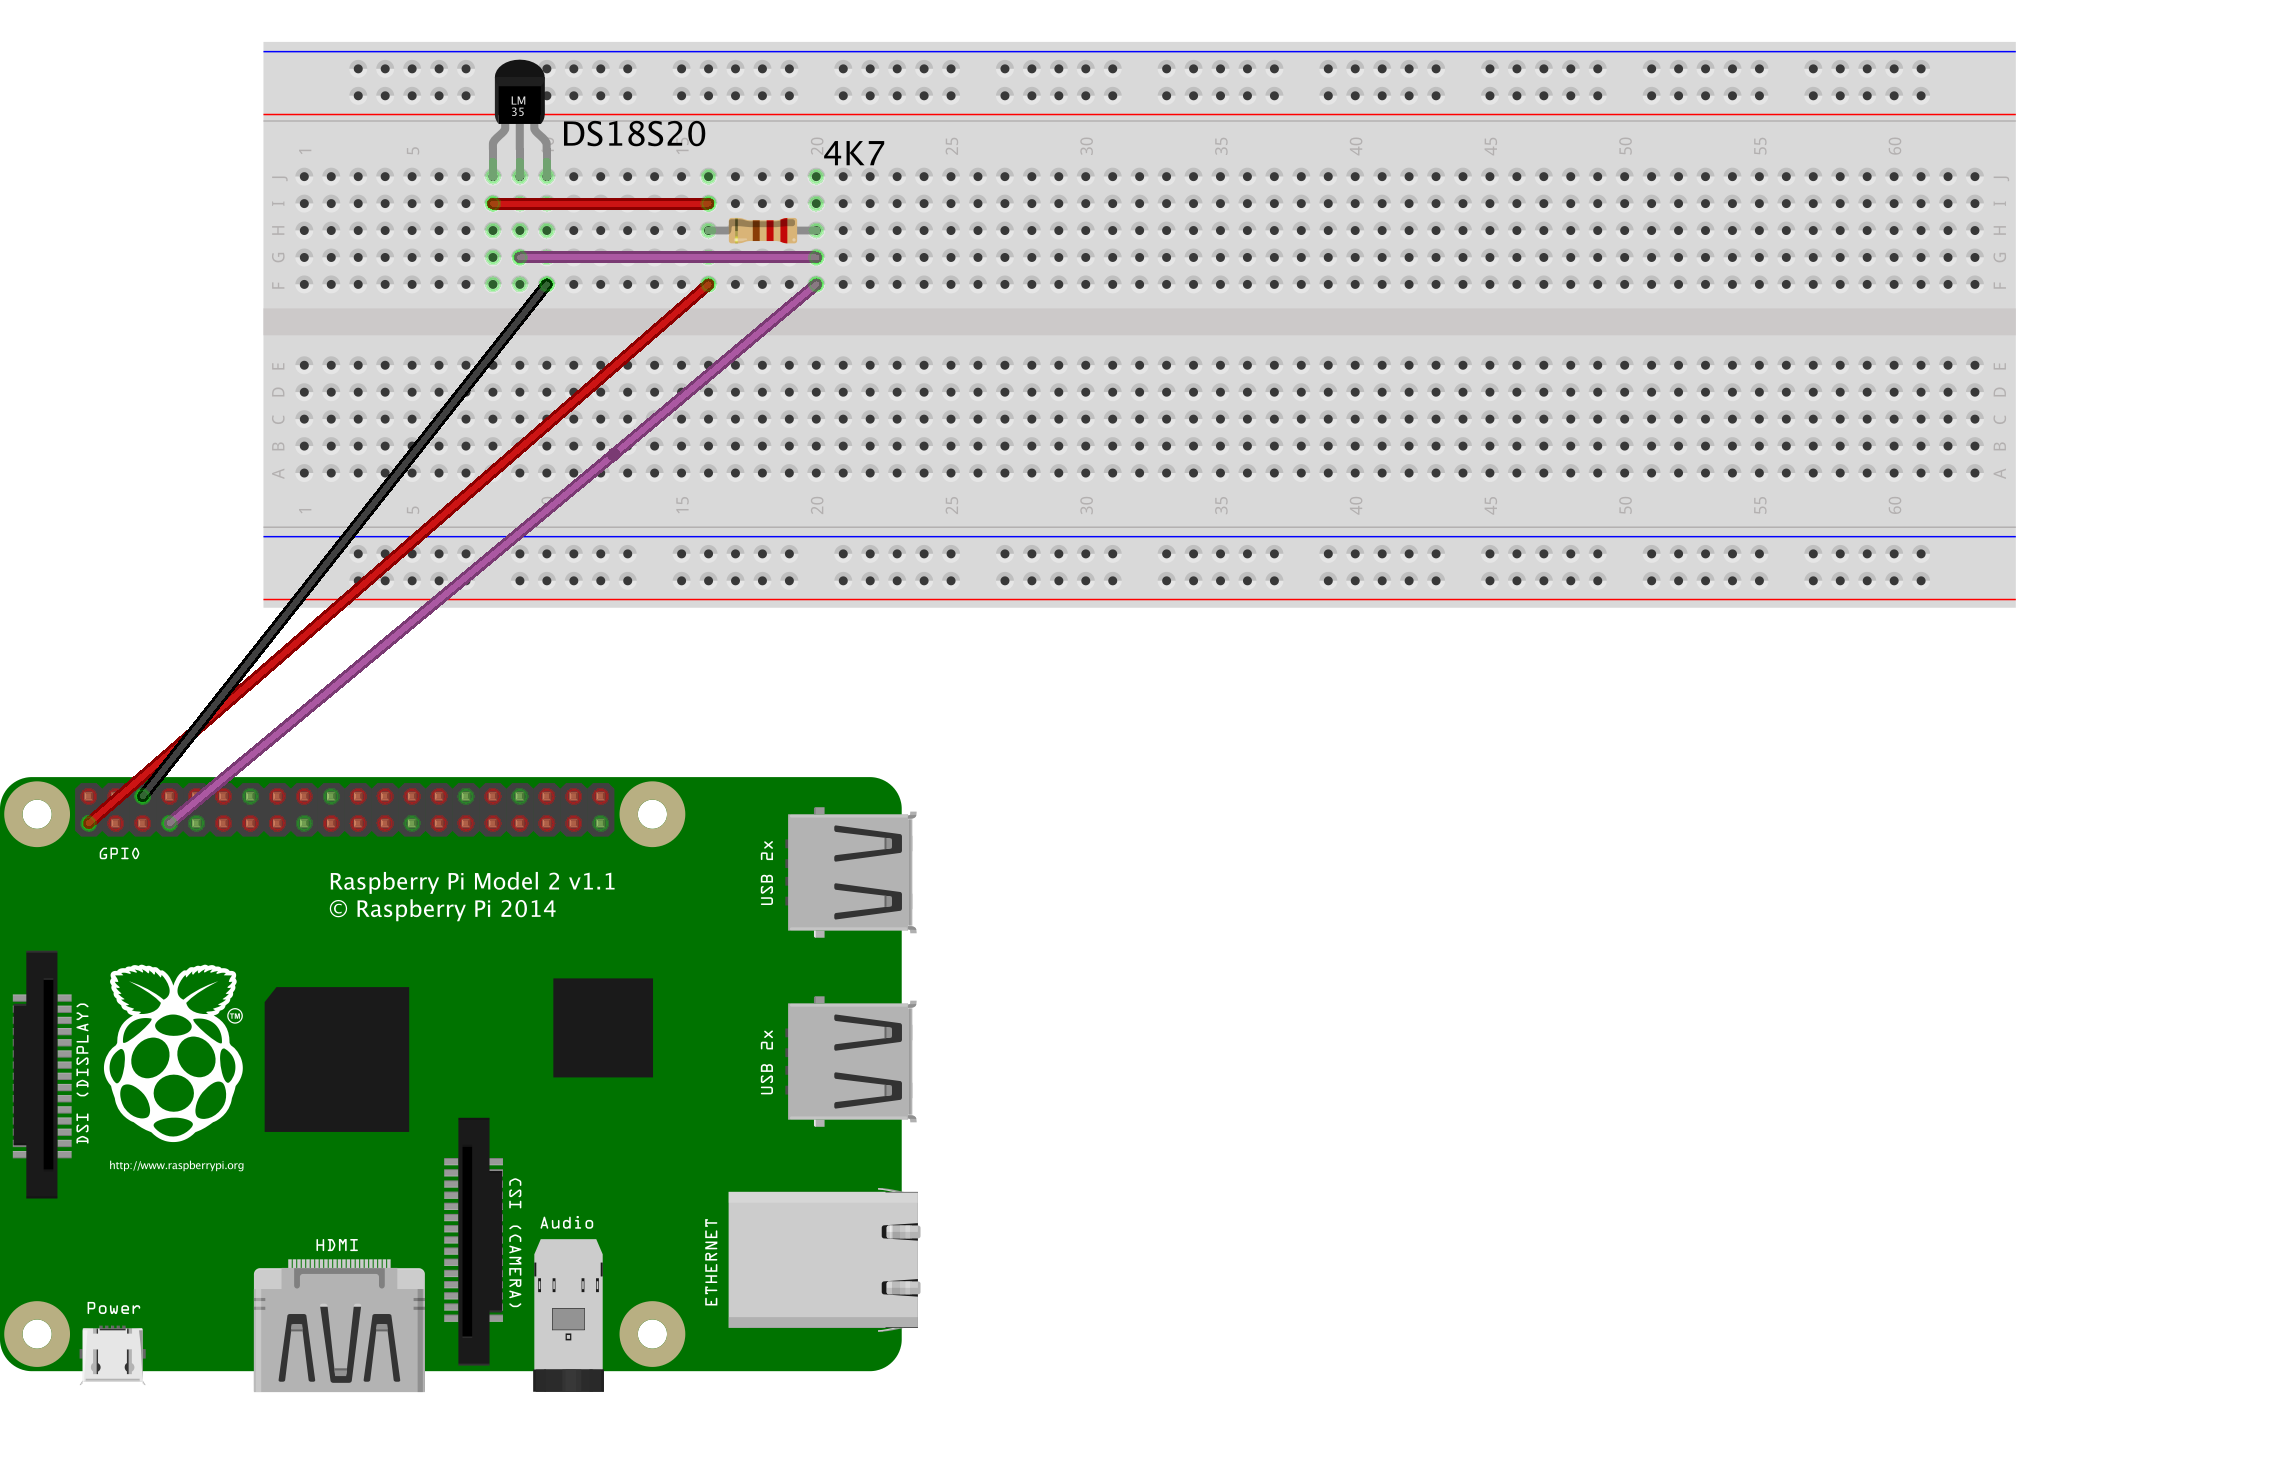
\includegraphics[scale=.8]{BilderAllgemein/Schaltung_DS18S20.png}
  \caption{Schaltungsaufbau DS18S20}
  \label{Abb_Schaltung_DS18S20}
\end{figure}

Die oben dargestellte Schaltung\footnote{gezeichnet mit Fritzing} zur Temperaturmessung wird folgendermaßen realisiert, der Pin $V_{DD}$ des Sensors ist mit Pin\,1 (3,3\,V) des \ac{RPI}\,3 verbunden (rote Verbindung). Die schwarze Verbindung stellt die GROUND Verbindung des Pin\,6 des \ac{RPI} mit dem GND Pin des Sensors dar. Weiterhin ist der er DQ Pin des Sensors (1-Wire Interface) mit dem Pin\,7 des \ac{RPI} verbunden (violette Verbindung). Der Pin\,7 des \ac{RPI} wurde für die Verwendung als 1-Wire Bus konfiguriert. Parallel zu dem  $V_{DD}$ und DQ Pin ist ein Pullup Widerstand geschalten.

\subsection{Auslesen des Sensors}
\label{subsection_Auslesen_DS18S20}
Um die vom Sensor erfassten Daten auf dem \ac{RPI}\,3 auszulesen, wird ein Python Script verwendet. Dieses wird im Anschluss an Hand kurzer Ausschnitte aus dem Quellcodes erklärt. Der komplette Quellcode ist im Anhang \ref{Python Script DS18S20} zu finden.\\

%Quellcode DS18S20
\lstset{escapeinside={\%*}{*},numbers=left,stepnumber=1}
\lstinputlisting[language=Python, firstline=16, lastline=32, caption=Auslesen der gemessenen Temperatur, label=list_DS18S20]{Listings/DS18S20/DS18S20.py}

Um die Temperatur des Sensors auslesen zu können wird in Zeile 2 des Codes das File geöffnet und dessen Inhalt in eine Variable gespeichert. Dieses File enthält die IDs, der an den \ac{RPI}\,3 angeschlossenen 1-Wire Sensoren. Jeder dieser Sensoren besitzt im Pfad \texttt{/sys/bus/w1/devices/} einen Ordner mit seiner ID. In diesem gibt es wiederum eine Datei mit der Bezeichnung \texttt{w1\_slave}, die die gemessenen Daten enthält. Um diese auszulesen, werden in dem Python Script in den Zeilen $8-15$ verschiedene Schritte durchgeführt, auf die nicht näher eingegangen wird\footnote{kann in verschiedenen Python Tutorials nachgelesen werden}. Da die Temperatur in der Datei im Format von z.B. 17687 ($\approx$ 17,7 $^\circ$C) angegeben wird, muss dieser Wert noch durch 1000 dividiert werden um den genauen Temperaturwert zu erhalten(Zeile 15 im Quellcode). In Zeile 16 wird der Wert noch auf zwei Stellen nach dem Komma gerundet und ist in der Variable \texttt{temperature} gespeichert. Mit dem Wert dieser Variable kann nun weiter gearbeitet werden.\\
Wichtig beim Auslesen der Dateien war es, darauf zu achten, dass die Temperaturwerte im richtigen Format ausgelesen werden, da es sonst im späteren Verlauf zu Problemen kommen kann (unübersichtliche Darstellung bei der Visualisierung).

%Subsection Datenspeicherung
\subsection{Datenspeicherung}
\label{subsectio_Datenspeicherung_DS18S20}
Wie schon in Abschnitt \ref{section_DS18S20} angesprochen, wird in diesem Teil der Arbeit auf die Möglichkeit der Datenspeicherung mittels RRDtool eingegangen. 

\subsection*{RRDtool}
Das RRDtool ist ein Programm, welches es ermöglicht, Messdaten für einen beim Erstellen festgelegten Zeitbereich zu speichern. RRD steht für \textit{Round-Robin-Database}, diese wird durch das Tool in einer Datei erzeugt, die von der Erstellung weg eine feste Größe besitzt. Dies ist ein großer Unterschied zu herkömmlichen mySQL Datenbanken, da bei diesen mit zunehmender Zeit und Datenmenge auch die Größe der Datenbank anwächst. Das Anwachsen der Größe der Datei wird bei der RRD Datenbank dadurch verhindert, dass sie wie ein Ringbuffer arbeitet, was bedeutet, dass wenn der Speicherplatz belegt ist, Werte zusammengefasst (z.B. durch Bildung eines Mittelwertes für einen Tag aus den einzelnen stündlichen Werten) und die ältesten überschrieben werden. Somit kann sichergestellt werden, dass die Größe der Datenbank schon beim Erstellen dieser festgelegt ist.\\
Wie eine solche Datenbank definiert und erstellt wird, wird im Quellcode \ref{list_Quellcode_RRD_Datenbank} beschrieben. Zum Erstellen der Datenbank wurde ein Shell-Script verwendet um nicht jedes Mal wenn die Datenbank neu erstellt wird alle Befehle einzeln eingeben zu müssen.

\subsection*{Erstellen der Datenbank}
\label{subsection_Erstellen_DB_DS18S20}
%Quellcode DS18S20
\lstset{escapeinside={\%*}{*},numbers=left,stepnumber=1}
\lstinputlisting[language=Python, firstline=1, lastline=9, caption=Erstellung RRD Datenbank , label=list_Quellcode_RRD_Datenbank]{Listings/DS18S20/RRD_DB_Erstellen.sh}

Um eine Datenbank zu erstellen, wurde in Zeile 2 des in \ref{list_Quellcode_RRD_Datenbank} dargestellten Source Codes der Name des zu erstellenden Datenbank Files festgelegt. Weiterhin wurde die Schrittweite\footnote{Datenbank erwartet alle 60 Sekunden einen Wert} auf \textit{60 Sekunden} festgelegt. Die nächsten Zeile definiert die Datenreihe, die Zahlen am Ende der Zeile legen fest, dass wenn innerhalb von 120 Sekunden kein gültiger Wert geliefert wird, die Datenbank an dessen Stelle \textit{NAN} (Not A Number) einträgt. Die Begründung liegt darin, dass wenn im weiteren Verlauf Mittelwerte etc. gebildet werden keine Verfälschung der Daten erfolgt (würde passieren wenn z.B. 0 eingetragen wird). In Zeile 4 wird der Zeitbereich der Speicherung von den gelieferten Werten definiert. Festgelegt wurde, dass jede Minute ein Wert gespeichert wird und dies 600 Minuten ($\approx$ 10 Stunden) lang.  Die Zeilen 5-9 des Quellcodes dienen dazu um die Bereiche von Maximl- bzw. Minimalwerten, sowie die Zeitspannen wann älteren Datenwerte zusammengefasst werden zu definieren. Genauere Informationen bezüglich der Erstellung der Datenbank können von folgender Adresse bezogen werden \url{http://oss.oetiker.ch/rrdtool/} \citep{Hompage_RRDtool}.\\\\
Das in Quellcode \ref{list_Quellcode_RRD_Datenbank} dargestellte Script musste nach dem speichern noch ausführbar gemacht werden. Dabei ergab sich das Problem, dass dieses beim Aufrufen die Datenbank wegen einer fehlenden Berechtigung nicht erstellen konnte. Dies wurde dadurch behoben, dass in Zeile 1 des Scripts der Aufruf des rrdtool mit \textit{sudo} realisiert wurde. Mit dem erfolgreichen Ausführen des Scripts wurde die Datenbank im Verzeichnis \texttt{/home/pi/Temperatur/TemperaturSensor/} angelegt.

\subsection*{Datenspeicherung}
\label{subsection_Speicherung der Daten des DS18S20}
Damit die über das Python Script ausgelesenen Daten in die Datenbank geschrieben werden, wurde am Ende des Scriptes folgende Zeile hinzugefügt.

\lstset{escapeinside={\%*}{*},numbers=left,stepnumber=1}
\lstinputlisting[language=Python, firstline=25, lastline=27, caption=Datenspeicherung in DB]{Listings/DS18S20/DS18S20.py}

Durch diese Codezeile, wird ein Update der Datenbank durchgeführt und der Wert, der in der Variable \texttt{temperature} gespeichert ist in diese geschrieben.
\newpage

%Subsection Visualisierung
\subsection{Visualisieren der Daten}
\label{subsection_Visualisieren der Daten DS18S20}
Die grafische Darstellung der Daten wurde wieder mit dem RRDtool realisiert. Hier wurden zwei Grafen erstellt die die gemessenen Temperaturwerte für verschiedene Zeiträume darstellen. Zur Erstellung dieser Grafen wurde ein Shell Script verwendet, das den entsprechenden Code enthält. Der Quellcode zur Erstellung der Graphen ist im Anhang dargestellt. Die einzelnen Befehle können auf folgender Quelle nachgeschlagen werden \url{http://oss.oetiker.ch/rrdtool/doc/rrdgraph_data.en.html}.\\
\\Abbildung \ref{Abb_Temperaturverlauf_Stunde_DS18S20} und \ref{Abb_Temperaturverlauf_10Stunden_DS18S20} zeigen die mittels RRDtool erzeugten Graphen.

%RRD Graphen
\begin{figure}[!h] 
  \centering
     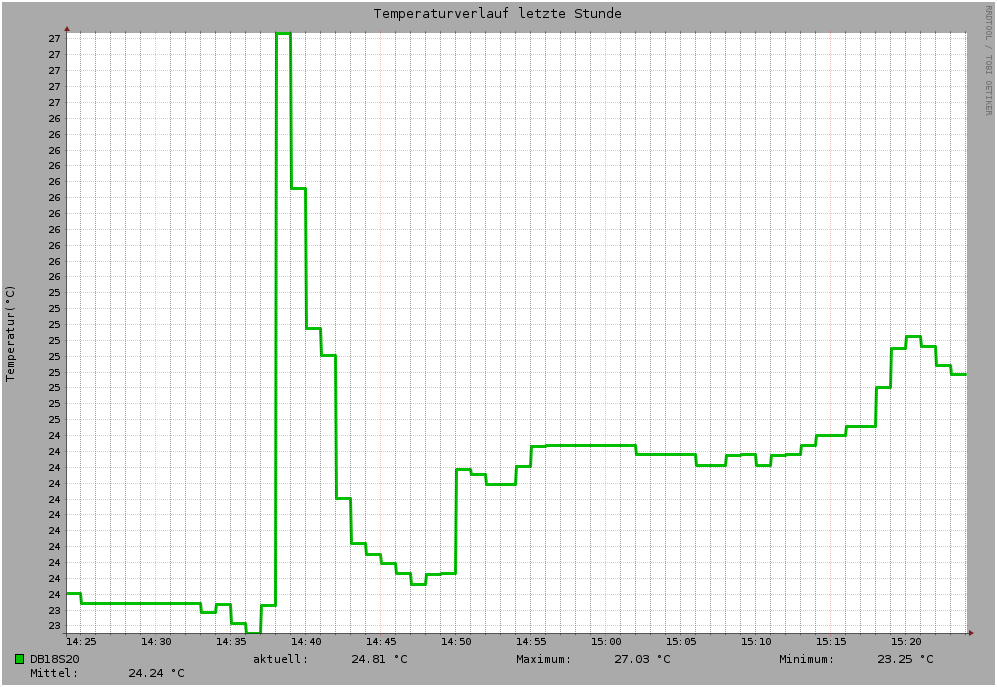
\includegraphics[scale=.28]{BilderAllgemein/TemperaturStunde.png}
  \caption{Temperaturverlauf der letzten Stunde}
  \label{Abb_Temperaturverlauf_Stunde_DS18S20}
\end{figure}

\begin{figure}[!h] 
  \centering
     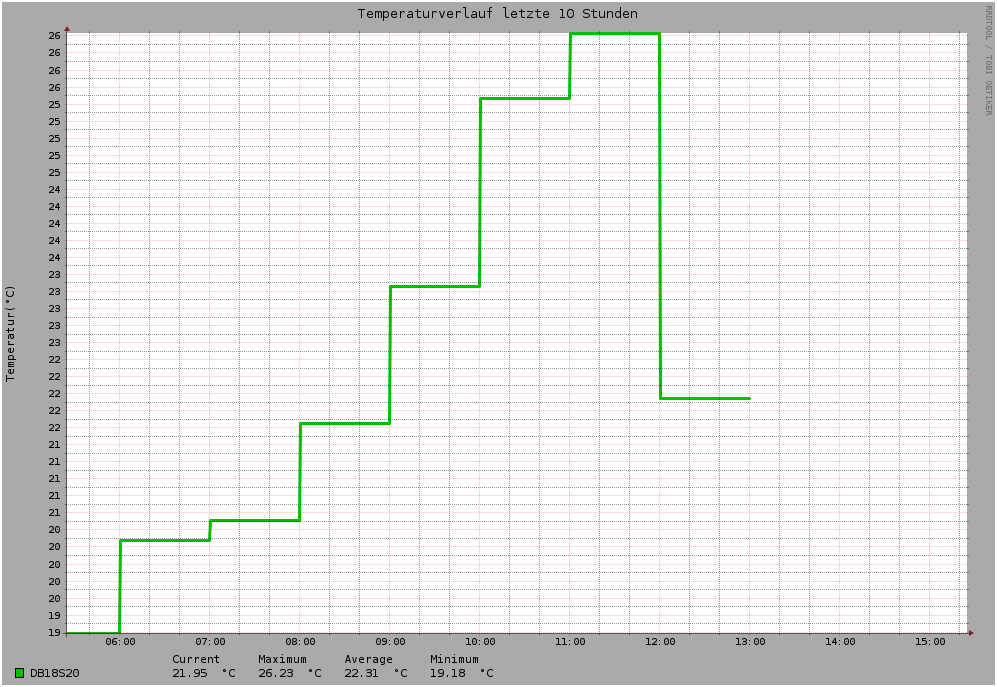
\includegraphics[scale=.28]{BilderAllgemein/TemperaturTag.png}
  \caption{Temperaturverlauf der letzten 10 Stunden}
  \label{Abb_Temperaturverlauf_10Stunden_DS18S20}
\end{figure}

Um die in diesem Versuch verwendeten Scripte zum Auslesen der Daten, Speichern der Daten oder Erstellung der Graphen für den Temperaturverlauf nicht immer von \glqq Hand\grqq ausführen zu müssen, wurde für jedes dieser Scripte ein extra Eintrag in der Datei \texttt{crontab\footnote{Cron-Daemon = Dienst der automatisch Scripte zu vorgegebenen Zeiten starten kann}} vorgenommen. Die Zeit wurde jeweils auf 1 Minute eingestellt.\\
Durch die Erstellung der oben aufgelisteten Graphen war es möglich den Temperaturverlauf im gemessenen Zeitraum nachzuverfolgen. Der Zeitraum der Messungen wurde über mehrere Tage ausgedehnt, damit eine realistische Temperaturaufzeichnung ausgewertet werden konnte. An Hand der erhaltenen Graphen konnten diverse Rückschlüsse gezogen werden (z.B. sank die Temperatur morgens um sechs Uhr jeweils um zwei Grad ab was über mehrere Tage nachzuverfolgen war. Dies lag daran, dass um diese Uhrzeit immer die Fenster geöffnet wurden).\\



%%%%%%%%%%%%%%%%%%%%%%%%%%%%%%%%%%%%%%%%%%%%%%%%%%%%%%%%%%%%%%%%%%%%%%%%%%%%%%%%%%%%%%%%%%%%%%%%%%%%%%%
%Abschnitt HYT-221
\section{Temperatur- und Luftfeuchtigkeitsmessung mit HYT-221}
\label{section_HTY221}
Bei diesem Versuchsaufbau, kommen im Gegensatz zu dem Aufbau in Abschnitt \ref{section_DS18S20} zwei weiter Sensoren hinzu. Zum Einen wird ein weiterer DS18S20 verbaut und zum Anderen ein HYT-221. Diese drei Sensoren werden gleichzeitig betrieben und liefern so eine gute Möglichkeit die Temperaturwerte zu einer bestimmten Zeit an Hand von unterschiedlichen Sensoren zu vergleichen.
\subsection{HYT-221}
\label{subsection_HYT221}
Der HYT-221 ist ein Sensor zur Messung der Temperatur und Luftfeuchtigkeit. Er wurde von der Schweizer Firma \ac{IST} für die Anwendung in den Bereichen Meteorologie, Industrielle Trocknungstechnik, Medizinische Geräte, Luftfahrt und Extremsport entwickelt. Der Sensor kommuniziert über eine \ac{I$^2$C} Schnittstelle und besitzt eine hohe Messgenauigkeit. In Tabelle \ref{Tabelle_Technische_Daten_HYT221}  werden die wichtigsten Daten des Sensors aufgelistet. Diese wurden dem Sensor zugehörigen Datenblatt entnommen \citep{Datenblatt_HYT221}.

%Tabelle Technische Daten HYT-221
\begin{table}[H]
%\rowcolors{2}{black!10}{black!20}
\centering
\begin{tabular}{
llll
}
\toprule
\multicolumn{2}{p{7cm}}{\centering\textbf{Feuchtemessung}} & \multicolumn{2}{p{7cm}}{\centering\textbf{Temperaturmessung} } \\
\multicolumn{1}{p{4cm}}{\textit{Bezeichnung}} & \multicolumn{1}{p{3cm}}{\centering\textit{Werte} }&\multicolumn{1}{p{4cm}}{\textit{Bezeichnung}} & \multicolumn{1}{p{3cm}}{\centering\textit{Werte} }\\\midrule
Messbereich & 0\dots 100\,\% rF & Messbereich  & -40\dots +125 $^\circ\text{C}$ \\
&&&\\
Genauigkeit & $\pm$ 1,8\,\% rF& Genauigkeit & $\pm$ 0,2 $^\circ\text{C}$\\
&&&\\
Auflösung & 0,02\,\% rF & Auflösung & 0.015 $^\circ\text{C}$\\
\bottomrule
\end{tabular}
\caption{Technische Daten HYT-221 \citep{Datenblatt_HYT221}}
\label{Tabelle_Technische_Daten_HYT221}
\end{table}



%Abbildung  HYT221
\begin{figure}[!h] 
  \centering
     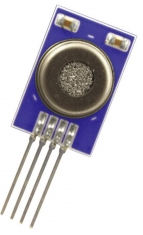
\includegraphics[scale=.4]{BilderAllgemein/HYT221.png}
  \caption{HYT-221 \citep{Bild_HYT221}}
  \label{Abb_HYT221}
\end{figure}

Für einen sicheren Betrieb des Sensors muss die angelegte Versorgungsspannung zwischen 2,7\dots 5,5\,$V$ liegen.

\subsection{Schaltungsaufbau}
\label{subsection_Schaltungsaufbau_HYT221}
Der in Abbildung dargestellte Schaltungsaufbau beinhaltet zwei Sensoren des Typs DS18S20, welche mit dem 1-Wire Bus betrieben werden. Der in Kapitel \ref{subsection_Schaltungsaufbau_DS18S20} erwähnte Pull-Up Widerstand wird dafür allerdings nur einmal benötigt, da beide Sensoren parallel zueinander geschalten sind. Als dritter Sensor ist ein HYT-221 verbaut, welcher Temperaturwerte und die Luftfeuchtigkeit misst. Der HYT-221 wird über den \ac{I$^2$C} Bus betrieben. Für diesen wurde eine $3,3\,V$ Versorgungsspannung (rote Verbindung), ein GROUND Anschluss (schwarze Verbindung), sowie zur Datenübertragung eine Taktleitung (SCL = rote Verbindung) und eine Datenleitung (SDA = blaue Verbindung) benötigt. Beim Aufbau dieser Schaltung war es wichtig, eine einheitliche Verkabelung der einzelnen Komponenten sicherzustellen (rote Verbindungen für 3,3\,V, schwarz für Ground etc.), um die Übersichtlichkeit zu bewahren. Ebenso musste darauf geachtet werden, dir Richtigen Pins miteinander zu verbinden, da die Fehlersuche ansonsten aufwendig werden würde.

%Abbildung Schaltungsaufbau HYT221
\begin{figure}[!h] 
  \centering
     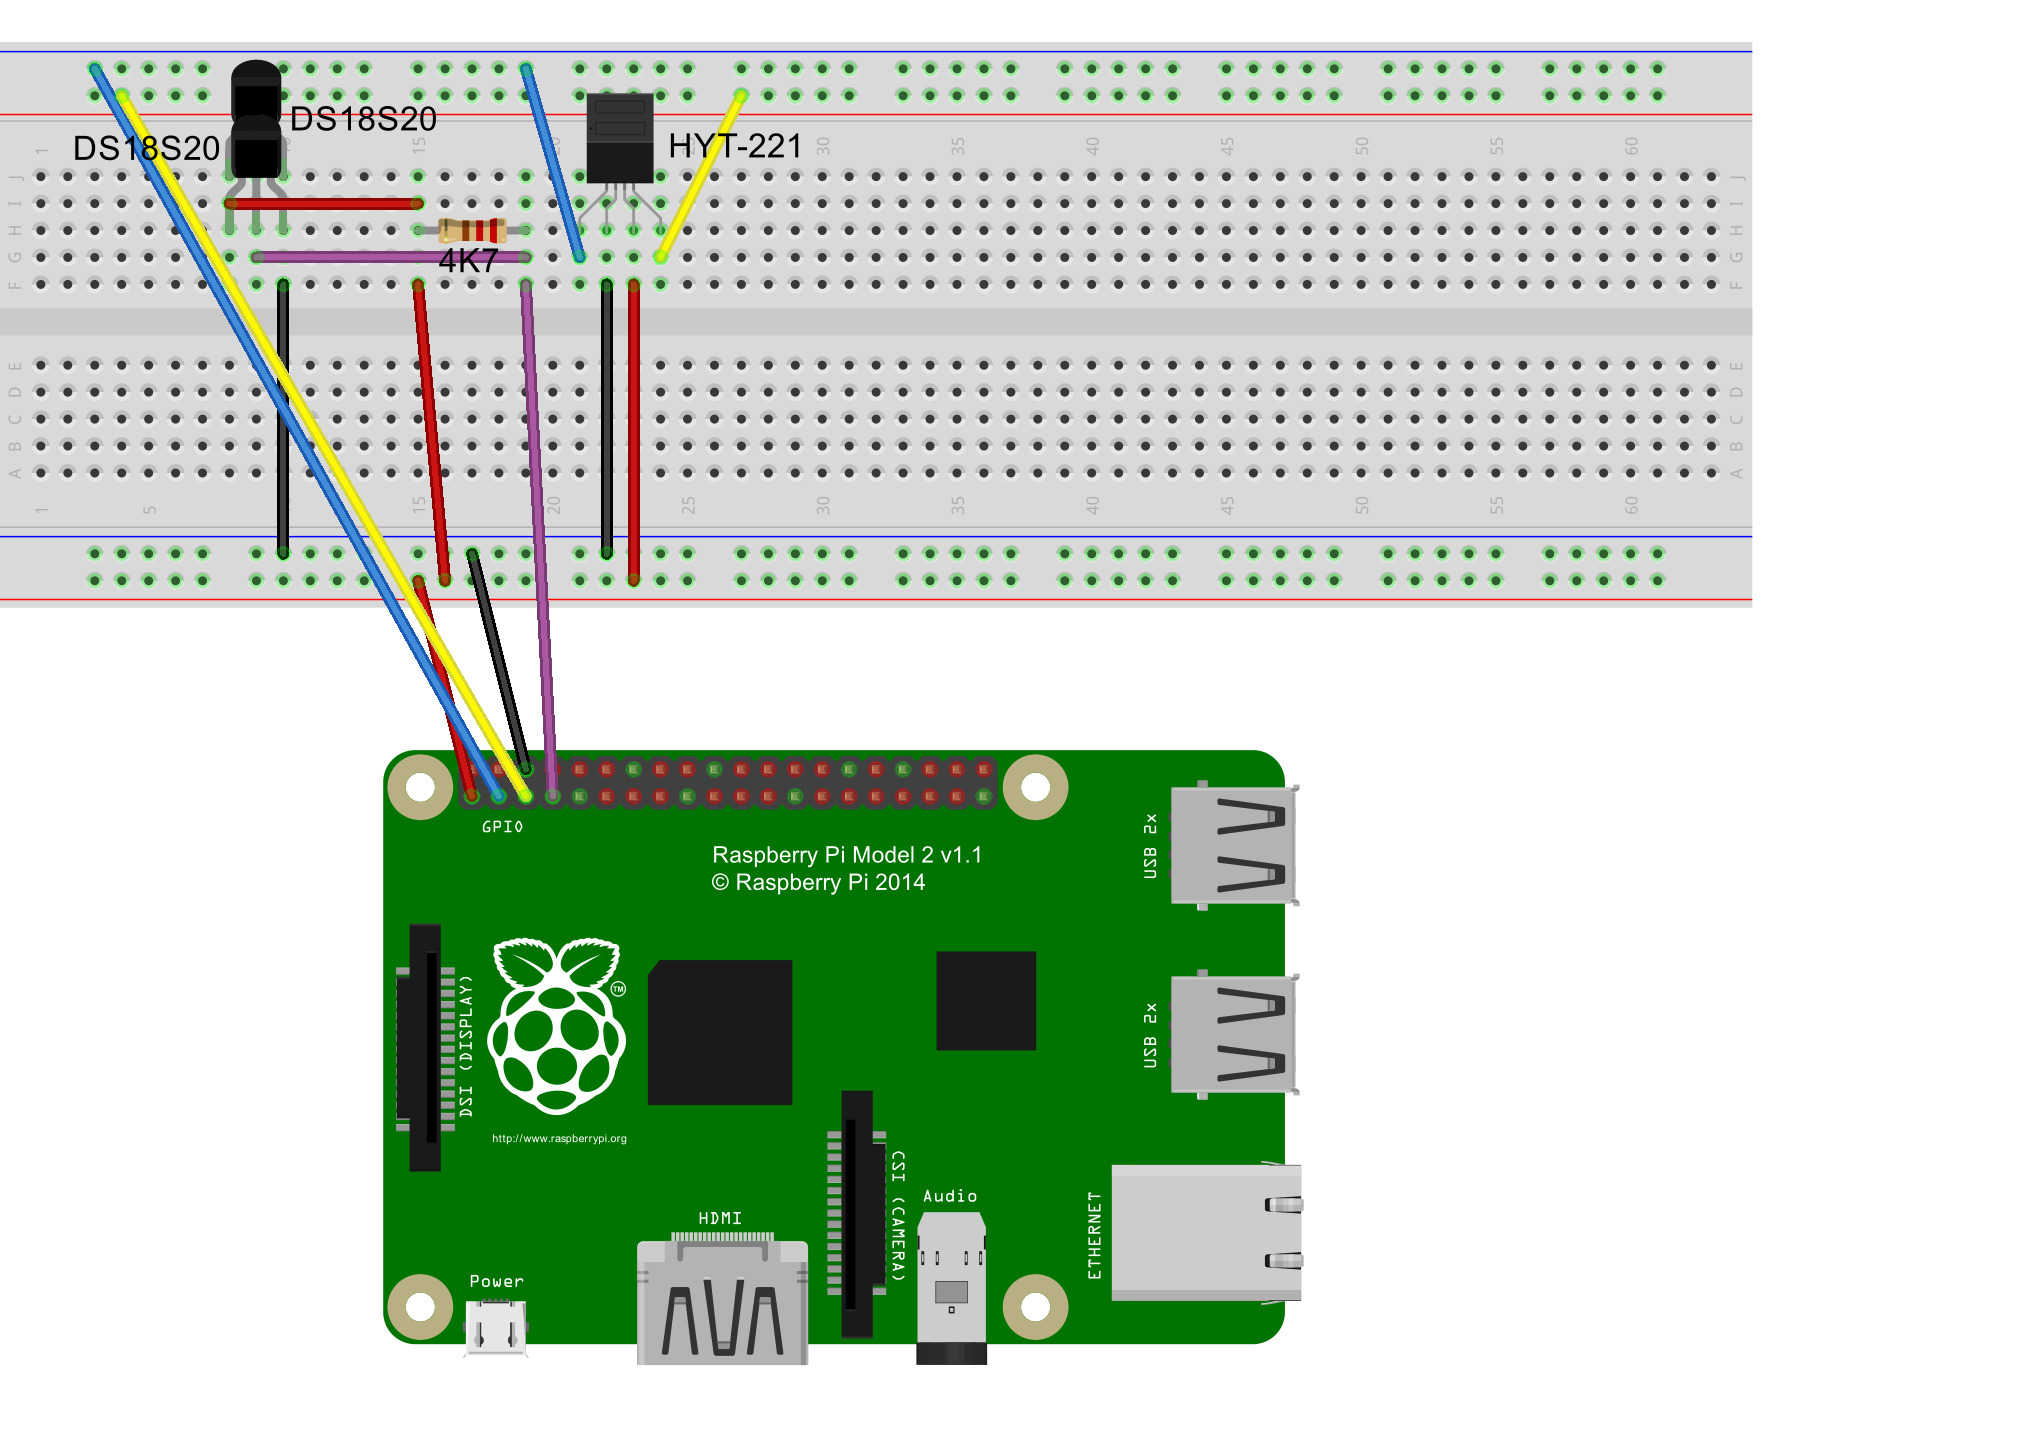
\includegraphics[scale=.72]{BilderAllgemein/Schaltung_HYT221.png}
  \caption{Schaltungsaufbau mit drei Sensoren}
  \label{Abb_Schaltungsaufbau_HYT221}
\end{figure}

%Subsection Auslesen der Daten HYT221
\subsection{Auslesen der Daten}
\label{subsection_Auslesen der Daten HYT221}
Im folgenden Code wurde das Auslesen der Daten des HYT-221 über den \ac{I$^2$C} Bus realisiert. Das Auslesen der Daten der beiden anderen Sensoren erfolgt analog zu der in Abschnitt \ref{subsection_Auslesen_DS18S20} dargestellten Möglichkeit, daher wird darauf nicht mehr explizit eingegangen. Der komplette Source Code ist in Anhang dargestellt.

\lstset{escapeinside={\%*}{*)},numbers=left}
\lstinputlisting[language=Python, firstline=20, lastline=45, caption=Auslesen der Temperatur und Luftfeuchtigkeit]{Listings/HYT221/Messung.py}

Um das Auslesen der Daten einfach zu gestalten, wurde im Script die Bibliothek \textit{smbus} importiert, welche fertige Funktionen zum Auslesen eines \ac{I$^2$C} Busses bereitstellt.\\
Als erstes wurde eine Variable mit der Adresse des Sensors angelegt. Diese Adresse kann dem Datenblatt des Sensors entnommen werden oder über den Befehl \texttt{i2cdetect -y 1} in der Konsole des \ac{RPI}\,3 ausgelesen werden. Der Parameter -y bewirkt, dass der Befehl sofort ausgeführt wird, der Parameter 1 legt fest das es sich um den \ac{I$^2$C} Bus Nummer 1 handelt (andere Hardware kann auch mehrere \ac{I$^2$C} Busse besitzen).\\
Um den smbus verwenden zu können musste ein Objekt dessen erzeugt werden (Zeile 13), die 1 in der Funktion steht wie schon beschrieben für den Bus Nummer 1. Im Anschluss wurde das erzeugte Array zur Speicherung der Daten noch initialisiert. Die Funktion in Zeile 22 erzeugt die im Theorie Teil beschriebene Startbedingung. Im Anschluss an die Startbedingung werden mit der Funktion \texttt{read\_i2c\_block\_data()} die Register, in denen die Werte für die Temperatur und Luftfeuchtigkeit gespeichert sind ausgelesen und in das Array gespeichert. Die Temperatur- und Feuchtigkeitswerte sind in vier Byte aufgeteilt und müssen dementsprechend nacheinander ausgelesen werden. Dies kann in der Protokollbeschreibung für den Sensor in folgender Quelle nachgelesen werden \citep{Datenblatt_I2C_HYT221}. Die übertragenen Werte, mussten im Anschluss an Hand von bestimmten Formeln, die dem Datenblatt des Sensors entnommen wurden in die jeweils richtige Form umgerechnet werden, um diese korrekt weiterverarbeiten zu können.

\subsection{Datenspeicherung}
\label{subsection_Datenspeicherung_HYT221}
Wie schon in Abschnitt \ref{subsection_Speicherung der Daten des DS18S20} beschrieben, wurden die Daten wieder in eine RRD Datenbank gespeichert. Der Source Code hierfür ist in Anhang \ref{Python Script HYT-221 mit RDD} abgebildet.\\
Weiterhin wurden die Sensordaten in einer mySQL Datenbank abgelegt, um die Möglichkeit zu schaffen, zu einem späteren Zeitpunkt durch exportieren dieser Daten (z.B. als CSV-File) eine weitere Bearbeitung zu ermöglichen. Möglichkeiten hierfür wären z.B. bei einer Fehlproduktion zu einem bestimmten Zeitpunkt (der die Aufzeichnungszeit des RRDtools übersteigt) eine Aussage über eventuelle Faktoren die dafür verantwortlich sein könnten tätigen zu können.\\
Der Source Code zur Realisierung der Datenspeicherung mittels mySQL DB ist im Anschluss aufgeführt. Die entsprechende DB wurde zuvor auf dem \ac{RPI}\,3 erstellt. Zur einfacheren Nutzung der mySQL Datenbank in dem Python Script wurde die Bibliothek \texttt{mysql.connector} importiert. Diese stellt vordefinierte Funktionen für die Verbindung mit der DB zur Verfügung, sowie Funktionen zum Lesen und Schreiben in bzw. aus der DB. Die Herstellung einer Verbindung zur Datenbank ist in Listing \ref{Datenbankverbindung} zu sehen.
Wichtig dabei war, die korrekten Anmeldedaten für die Datenbank zu verwenden, da ansonsten die Verbindung nicht hergestellt werden konnte und eine Fehlermeldung ausgegeben wurde.

\lstset{escapeinside={\%*}{*)},numbers=left}
\lstinputlisting[language=Python, firstline=12, lastline=17, caption=Verbindung zur DB herstellen,label=Datenbankverbindung]{Listings/HYT221/Messung.py}

Um auf die Tabelle in der Datenbank zugreifen zu können musste noch ein Cursor erzeugt werden (Zeile 4). An Hand von SQL Statements wurden dann die Daten in die entsprechenden Spalten der Tabelle eingefügt (Zeile 9-10 und Zeile 13-14). Damit die Änderungen in der Tabelle gespeichert werden, musste in Zeile 16 noch ein commit durchgeführt werden. Am Ende wurde die Verbindung zu Datenbank wieder geschlossen.

\lstset{escapeinside={\%*}{*)},numbers=left}
\lstinputlisting[language=Python, firstline=95, lastline=112, caption=Speicherung der Daten in mySQL DB]{Listings/HYT221/Messung.py}

\subsection{Visualisierung der Daten}
\label{subsection_Visualisierung der Daten}
Die Messdaten wurden wie im Abschnitt \ref{subsection_Visualisieren der Daten DS18S20} mit dem RRDtool visualisiert. Hier wurden die Werte aller drei Sensoren in den Graphen abgebildet, was einen Vergleich der Temperaturwerte zwischen den verschiedenen Sensoren recht leicht machte. Als Ergebnis konnte festgehalten werden, dass sich die Sensoren im Durchschnitt um maximal 0,5 Grad unterschieden haben. Dies spricht wiederum für die Messgenauigkeit der einzelnen verwendeten Sensoren. Auch wurde noch ein weiterer Graph für den Zeitraum von den letzten drei Tagen hinzugefügt. Die Graphen mit den Temperatur und Feuchtigkeitswerten sind im Anhang \ref{Anhang_Abbildung_Temperaturverlauf} aufgelistet. Ebenso ist der Quellcode für die Erstellung der Graphen in \ref{Erstellung Graphen HYT-221}  ersichtlich.\newpage


%%%%%%%%%%%%%%%%%%%%%%%%%%%%%%%%%%%%%%%%%%%%%%%%%%%%%%%%%%%%%%%%%%%%%%%%%%%%%%%%%%%%%%%%%%%%%%%%%%%%%%%
\section{Vibrationsmessung mit Sensor BMA020}
\label{section_BMA020}
Im dritten Versuchsaufbau sollte mit dem Beschleunigungssensor BMA020 die Vibration gemessen werden. Verwendet wurde hier eine schon fertig bestückte Platine die den BMA020 enthält.

\subsection{BMA\,020}
\label{subsection_BMA020}
Der BMA\,020 ist ein von Bosch entwickelter Sensor, der die Beschleunigung in drei Richtungen (x-, y- und z-Achse) misst. Die Messdaten werden im Format eines 2er Komplements mit 10\,Bit ausgegeben. Als Schnittstellen stellt der BMA\,020 einen SPI- und \ac{I$^2$C} Bus zur Verfügung. Die wichtigsten technischen Daten wurden dem Datenblatt \citep{Datenblatt_BMA020} entnommen und in der Tabelle \ref{Tabelle_Technische_Daten_BMA020} dargestellt.  

%Tabelle Technische Daten HYT-221
\begin{table}[H]
%\rowcolors{2}{black!10}{black!20}
\centering
\begin{tabular}{
lll
}
\toprule

\multicolumn{1}{p{5.5cm}}{\textit{Parameter}} & \multicolumn{1}{p{3cm}}{\textit{Minimum} }&\multicolumn{1}{p{3cm}}{\textit{Maximum}}\\\midrule
&-2\,g & 2\,g\\
Acceleration range & -4\,g & 4\,g\\
&-8\,g & 8\,g\\
&&\\
Supply voltage analogue & 2\,V & 3,6\,V\\
&&\\
Acceleration output resolution &&10\,Bit\\
\bottomrule
\end{tabular}
\caption{Technische Daten BMA020 \citep{Datenblatt_BMA020}}
\label{Tabelle_Technische_Daten_BMA020}
\end{table}

Abbildung zeigt die fertig bestückte Platine mit dem BMA020.

%Abbildung  BMA020
\begin{figure}[!h] 
  \centering
     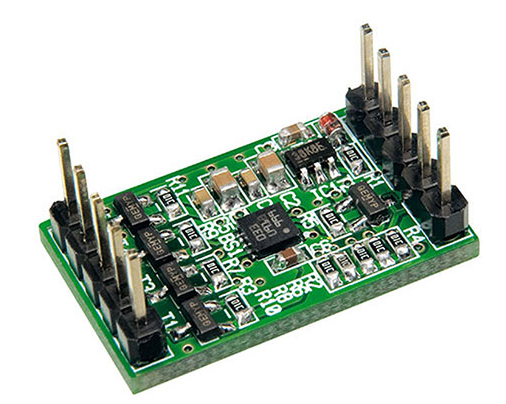
\includegraphics[scale=.4]{BilderAllgemein/Beschleunigungssensor.png}
  \caption{Platine mit BMA020 \citep{Bild_BMA020}}
  \label{Abb_HYT221}
\end{figure}
\newpage

\subsection{Schaltungsaufbau}
\label{subsection_Schaltungsaufbau_BMA020}

\begin{figure}[!h] 
  \centering
     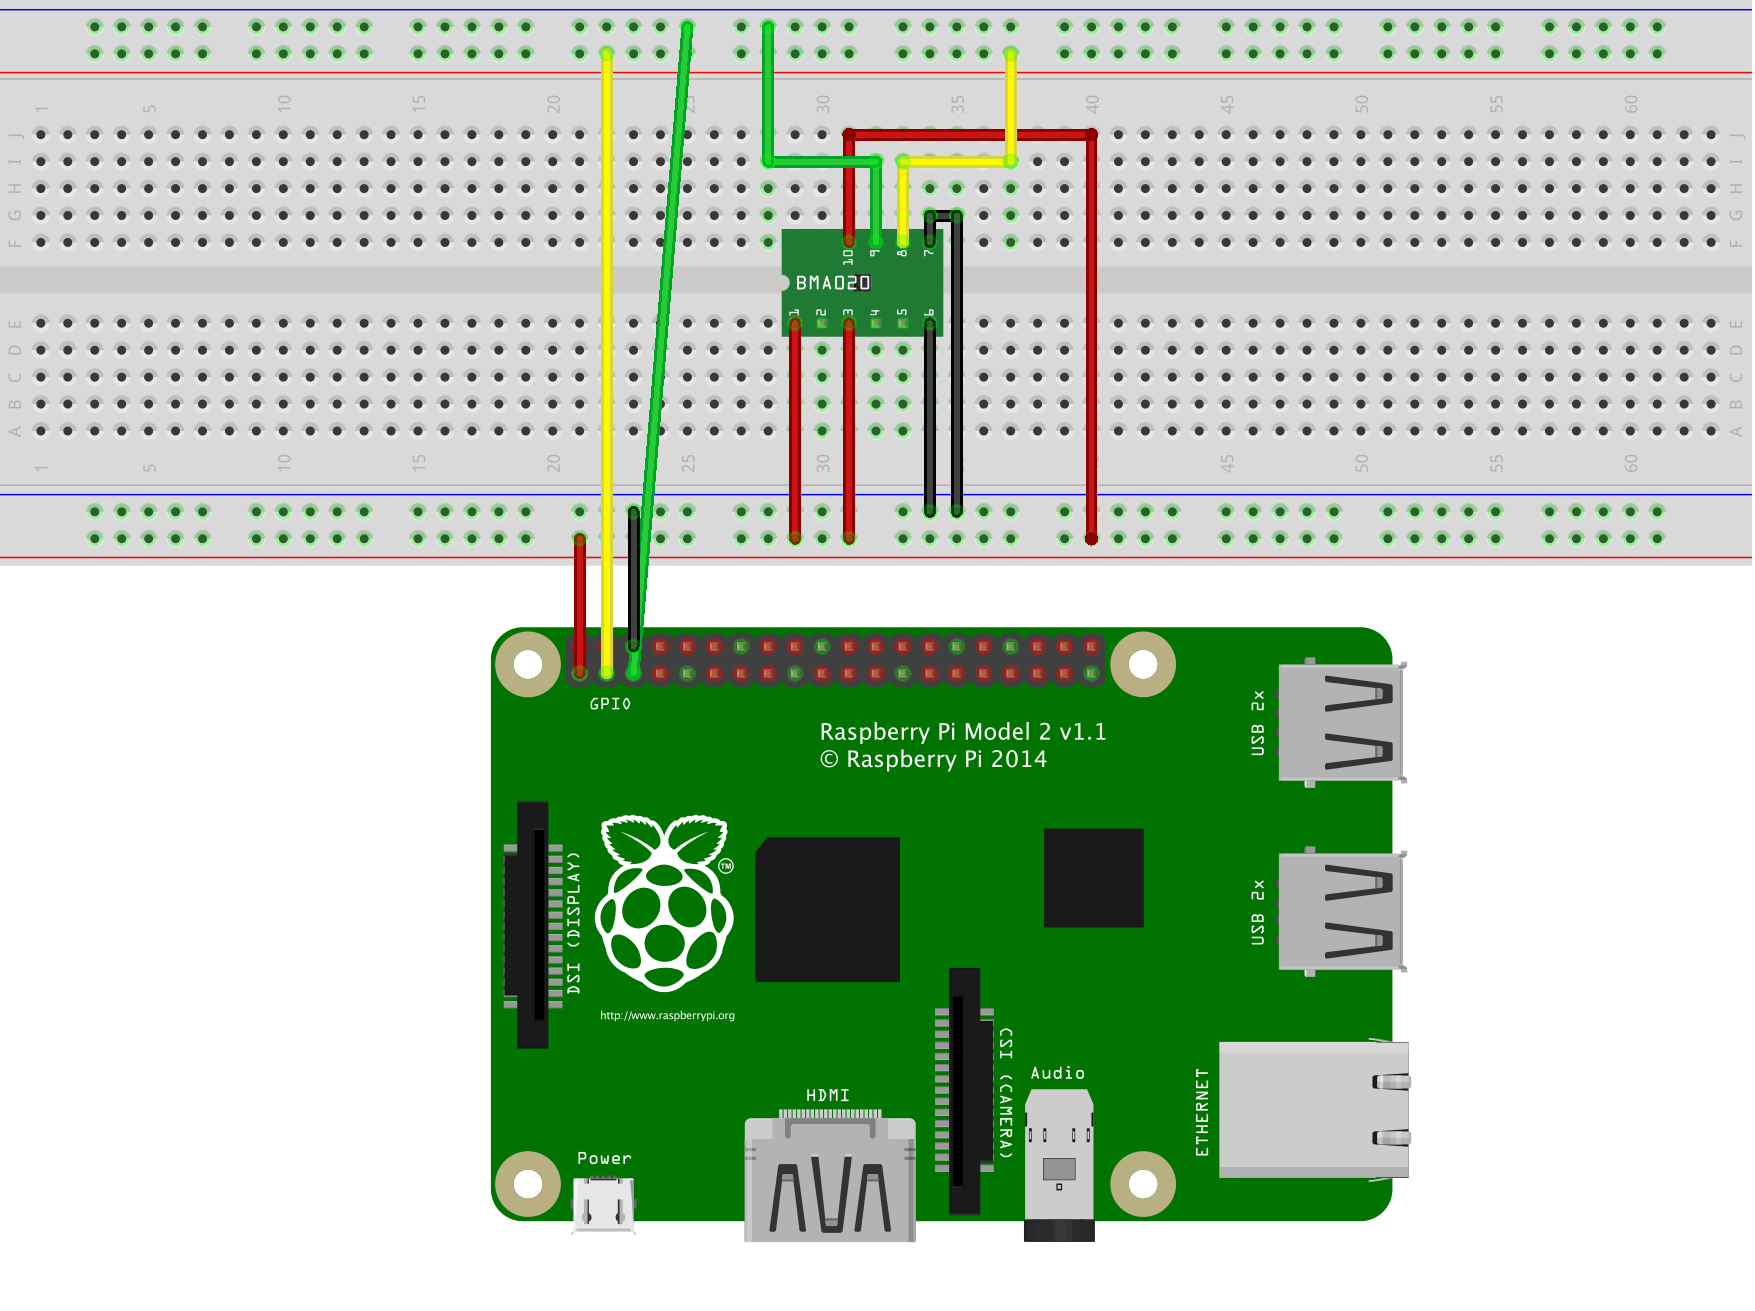
\includegraphics[scale=.8]{BilderAllgemein/Schaltung_Vib.png}
  \caption{Schaltungsaufbau Vibrationsmessung mit  BMA020}
  \label{Abb_Schaltungsaufbau_BMA020}
\end{figure}

Die in Abbildung \ref{Abb_Schaltungsaufbau_BMA020} dargestellte Schaltung beinhaltet die fertig bestückte Platine mit dem BMA020. Weiterhin ist auf der Platine auch ein Pullup Widerstand mit verbaut, sowie weitere Widerstände, um eine Spannungsversorgung der Platine mit 2,5\,V - 6\,V zu gewährleisten ohne dass der BMA020 Schaden nimmt (Spannungsversorgung des BMA\,020 liegt sonst bei max. 3,6\,V).\\
Die Schaltung wurde an Hand des Datenblattes der Platine für einen Betrieb mittles \ac{I$^2$C} Schnittstelle verdrahtet. Dafür wurde die Pins \textit{UIN, CSB} und \textit{UPULLUP} mit einer 3,3\,V Versorgungsspannung belegt (rote Verbindungen). Die Pins \textit{SDO} und \textit{GND} wurde auf GROUND gelegt (schwarze Verbindungen). Für die Datenübertragung wurde der Pin SCK mit dem SCL Pin des \ac{RPI} (grüne Verbindung), sowie der SDI Pin mit dem SDA Pin des \ac{RPI} (gelbe Verbindung) verbunden.

\subsection{Auslesen der Daten}
\label{subsection_Auslesen_Daten_BMA020}

Um die Daten über den \ac{I$^2$C} Bus auszulesen, wurde ähnlich vorgegangen wie bei der Temperatur- und Luftfeuchtigkeitsmessung. Die Änderung dazu war allerdings, dass das Python Script nicht wie zuvor über den Crown-Deamon jede Minute aufgerufen wurde sondern die Messungen in einer while Schleife jede Sekunde ausgewertet wurden. Dies war für die Aussage über eventuelle Vibrationen nötig, da ansonsten keine aussagekräftigen Werte ermittelt werden können.\\
Als erstes wurden die Funktionen zum Auslesen der Register und für die Umwandlung des 2er Komplements definiert (Zeile 30 - 43). In Zeile 45 - 47 ist die Funktion für die Startbedingung des \ac{I$^2$C} Busses definiert. In der folgenden while Schleife wurden dann mittels der vorher definierten Funktion die Register für die verschiedenen Beschleunigungsrichtungen ausgelesen. Hier mussten für jeden Beschleunigungswert zwei verschiedene Register gelesen werden, da die Werte in diesen gespeichert waren\footnote{im Datenblatt des Sensors ersichtlich} (für x-Achse musste z.B. das Register 0x02, das die LSB-Werte enthält und das Register 0x03 mit den MSB-Werten gelesen und entsprechend zusammengesetzt werden). Im Anschluss wurden noch die digitalen Werte in die entsprechnden g-Werte umgerechnet um eine aussagekräftige Darstellung zu ermöglichen. Der Ausschnitt für den eben beschrieben Teil des Source Codes ist in Listing \ref{Auslesen_Vibrationswerte_BMA020} ersichtlich. Der gesamte Quellcode ist in Anhang \ref{Python Script Vibrationsmessung} aufgelistet.

\lstset{escapeinside={\%*}{*)},numbers=left}
\lstinputlisting[language=Python, firstline=30, lastline=66, caption=Auslesen der Vibrationswerte,label=Auslesen_Vibrationswerte_BMA020]{Listings/Vibration/Vibration.py}

\subsection{Datenspeicherung}
\label{subsection_Speicherung_der_Vibrationsdaten}
Die Vibrationswerte der verschiedenen Bewegungsrichtungen wurden in diesem Testaufbau im Sekundentakt in einer mySQL Datenbank gespeichert. Die Werte wurden wie schon im vorherigen Beispiel über SQL Statements in die entsprechende Tabelle der Datenbank geschrieben. Zuvor wurde wieder die Verbindung zur DB über das Python Script hergestellt. Der genaue Ablauf ist im Quelltext im Anhang \ref{Python Script Vibrationsmessung} ersichtlich.

\subsection{Visualisierung der Vibrationswerte}
\label{subsection_Visualisierung der Vibrationswerte}
Im Gegensatz zu den vorherigen Beispielen, wurde in diesem Fall auf eine Visualisierung mittels Graphen verzichtet, da damit eine Vibrationsmessung in nahezu Echtzeit schwer zu realisieren war. Es hätte hierfür jede Sekunde ein Graph mit dem RDDtool erstellt werden müssen, was eine sehr große Systemlast zur Folge gehabt hätte.\\
Daher wurde die Auswertung über ein HTML File realisiert, welches mittels AJAX (Asynchronous JavaScript and XML) die aktuellen Beschleunigungswerte mit dem sich am Server befindenden PHP-Script austauscht. Das PHP-Script, das sich auf dem WebServer (wurde auf dem \ac{RPI} installiert) befindet, ließt die aktuellen Beschleunigungswerte aus einem Textfile aus. Die Daten in diesem Textfile wurden von dem Python Script in dieses geschrieben (Zeile 73 - 75 im Python Script). Die Darstellung der HTML Seite ist im Anhang \ref{Anhang_Visualisierung der Vibrationswerte} ersichtlich. Bei dieser Darstellung wurde noch darauf geachtet, dass bei nicht bedenklichen Beschleunigungswerten die Angaben in grüner Schrift, bei erhöhten Beschleunigungswerten in oranger Schrift und bei kritischen Beschleunigungswerten in roter Schrift dargestellt werden. Wenn nur ein Beschleunigungswert einer Richtung im kritischen Bereich liegt, so wird zusätzlich im unteren Bereich der Anzeige eine Warnmeldung eingeblendet. Dies Logik wurde über ein JavaScript File realisiert. Die verschiedenen Quelltexte der einzelnen Files sind im Anhang   \ref{PHP-Script zum Auslesen der Beschleunigungswerte} \ref{JavaScript File zur Visualisierung der Beschleunigungswerte} \ref{HTML File zur Darstellung der Beschleunigungswerte} aufgelistet. 